\documentclass[
	12pt,				% tamanho da fonte
	oneside,			% para impressão apenas no recto. Oposto a twoside
	a4paper,			% tamanho do papel. 
	% -- opções da classe abntex2 --
	%chapter=TITLE,		% títulos de capítulos convertidos em letras maiúsculas
	%section=TITLE,		% títulos de seções convertidos em letras maiúsculas
	%subsection=TITLE,	% títulos de subseções convertidos em letras maiúsculas
	%subsubsection=TITLE % títulos de subsubseções convertidos em letras maiúsculas
	% -- opções do pacote babel --
	english,			% idioma adicional para hifenização
	brazilian,				% o último idioma é o principal do documento
	]{article}

\usepackage[brazilian]{babel}		% Language-specific settings
\usepackage{fontspec}
\usepackage{indentfirst}		% Indenta o primeiro parágrafo de cada seção.
\usepackage{nomencl} 			% Lista de simbolos
\usepackage{color}				% Controle das cores
\usepackage{graphicx}			% Inclusão de gráficos
\usepackage{amsmath}
\usepackage{amssymb}
\usepackage{bm}
\usepackage{microtype} 			% para melhorias de justificação
\usepackage[
	top=3cm,
	bottom=2cm,
	left=3cm,
	right=2cm
]{geometry}
\usepackage{setspace}
\usepackage{csquotes}
\usepackage[
	backend=biber,	% Use Biber backend (more powerful than BibTex)
	style=ieee,
	backref=true
]{biblatex}
\usepackage{float}
\usepackage{caption}

\graphicspath{{images/}}


\setmainfont{Arial}
\onehalfspacing

\addbibresource{references.bib}

\title{\textbf{USO DE REDES NEURAIS PARA APROXIMAR OS PESOS DE INTERPOLAÇÃO DO SISTEMA HIG-FLOW}}
\author{}
\date{\today}


\begin{document}

	% Retira espaço extra obsoleto entre as frases.
	\frenchspacing 

	\maketitle

	\section{Introdução}

	Simular fluidos em malhas não estruturadas (irregulares) é um desafio, tanto em questão de modelagem, quanto na capacidade computacional necessária. Nesses casos, normalmente é necessário realizar interpolações geométricas, operações que são altamente dependentes das células ao redor do ponto desejado, o que impacta negativamente na complexidade dessa operação, principalmente em três dimensões. Com isso em mente, o trabalho de \cite{Sousa2019} propõe um método de diferenças finitas para malhas hierárquicas usando MLS (\textit{Moving Least Squares}), um método \textit{meshless}, para realizar as interpolações.

	No \textit{HiG-Flow}, software que implementa as ideias de \cite{Sousa2019} na linguagem de programação C, a malha hierárquica é armazenada em uma estrutura de dados chamada \textit{HiG-Tree} (\textit{Hierarchical Grid Tree}), uma árvore em que cada folha (célula) pode ser refinada geometricamente em subcélulas, dando origem a novas folhas, como pode ser visto na figura \ref{fig:higtree}.
	
	\begin{figure}[H]
		\centering
		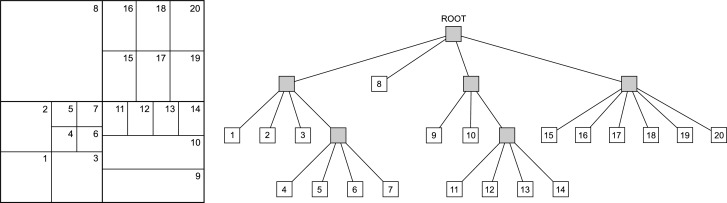
\includegraphics[width=0.8\textwidth]{higtree.jpg}
		\captionsetup{justification=centering}
		\caption{Exemplo da estrutura de dados higtree\\ Fonte: \cite{Sousa2019}}
		\label{fig:higtree}
	\end{figure}

	Note que, para usar as diferenças finitas clássicas, os pontos da malha devem estar organizados em retângulos (no caso 2D), o que nem sempre ocorre com uma malha hierárquica, tornando necessário as interpolações para pontos fora da malha. O método proposto por \cite{Sousa2019} é custoso computacionalmente, ao passo que para cada interpolação, um sistema deve ser resolvido. Isso não é um grande problema em malhas estáticas, já que o cálculo dessas interpolações pode ser feito como um passo de pré-processamento e os pesos de interpolação podem ser guardados em \textit{cache}.

	O desafio fica claro quando mudamos para uma malha dinâmica. Para cada passo de tempo da simulação, diversas interpolações devem ser calculadas, o que pode se tornar um gargalo em uma malha com milhões de células. 

	Atualmente, o sistema \textit{HiG-Flow} implementa a técnica \textit{PLIC-VOF} (Piecewise Linear Interface Calculation - Volume of Fluid) para simular escoamentos bifásicos \cite{Silva2025}. Além disso, estão sendo desenvolvidas ferramentas para o refinamento adaptativo da malha, principalmente ao redor das interfaces entre os fluidos. Nesses locais do domínio, é necessário uma malha mais fina, para evitar o \textit{smearing} (espalhamento) da interface e limitar melhor a fração de volume $f$ para $f \in [0,1]$ \cite{MARZIALE2025106794,MENCINGER2011644}.

	Com isso em mente, para tentar reduzir o gargalo computacional associado às interpolações, uma saída é utilizar redes neurais para inferir os pesos de interpolação da malha. No entanto, note que, para cada ponto onde os pesos devem ser calculados, há um valor variável de células adjacentes utilizadas.
	


	\section{Objetivos}

	O presente projeto tem como objetivo principal investigar, desenvolver e avaliar o uso de Redes Neurais Artificiais (RNAs), como um método eficiente e robusto para calcular os pesos de interpolação espacial no sistema de simulação de fluidos \textit{HiG-Flow}.

	Para o alcance do objetivo principal, definem-se os seguintes objetivos específicos:
	\begin{itemize}
		\item Desenvolver e treinar um modelo de rede neural que calcule os pesos de interpolação (como os gerados pelos Mínimos Quadrados Móveis - MLS), mantendo precisão numérica suficiente para não comprometer a convergência do método numérico
		\item Avaliar e otimizar a eficiência computacional do modelo desenvolvido, visando uma execução de inferência significativamente mais rápida do que o cálculo analítico matricial tradicional.
		\item Projetar uma metodologia de tratamento de dados que solucione o problema da dimensionalidade variável dos estênceis de malhas hierárquicas.
		\item Integrar a rede neural treinada nativamente à base de código em linguagem C do simulador \textit{HiG-Flow}.
	\end{itemize}


	\section{Plano de Trabalho e Cronograma}

	No primeiro trimestre, o aluno deve se familiarizar com o software \textit{HiG-Flow} (\cite{Sousa2019,Raymundo2024,Silva2025,HigFlowGitHub}), sendo capaz de realizar simulações e alterar o código quando pertinente. No segundo trimestre, deverá revisar técnicas de Machine Learning (tais como descritas em \cite{Goodfellow-et-al-2016,Braga2007,Haykin1999}), escolhendo qual tipo de rede neural deverá ser empregada, assim como a ferramenta utilizada.

	A partir do segundo semestre, o aluno se dedicará à implementação computacional do projeto. Dessa forma, deve treinar e testar a rede neural, assim como portabilizá-la para o \textit{HiG-Flow}.


	\section{Materiais e Métodos}

	Atualmente no \textit{HiG-Flow}, para cada ponto de um estencil que não corresponde a nenhum ponto da malha, é necessário executar uma interpolação. Seja $\mathbf{x}$ esse ponto fora da malha e suponha que queremos interpolar uma função $u:\mathbb{R}^d \to \mathbb{R}$ pelas funções linearmente independentes e suaves $\Phi_i:\mathbb{R}^d \to \mathbb{R}$, $i=1, \dots, n$ tal que a aproximação $U(\mathbf{x})$ seja dada por:
	\begin{equation}
		U(\mathbf{x}) = \sum_{j=1}^{n}c_j\Phi_j(\mathbf{x})
	\end{equation}
	Dados $m$ pontos da malha $x_1, \dots, x_m$ com $m > n$ e $u_i = u(x_i)$, $i=1,\dots,m$, definimos $\mathbf{u} = (u_1, \dots, u_m)$, $\mathbf{U} = (U(x_1), \dots, U(x_m))$, $\mathbf{c} = (c_1, \dots, c_n)$ e a função de erro
	\begin{equation}
		E(\mathbf{c}) = ||\mathbf{U} - \mathbf{u}||^2_2 = \sum_{i=1}^{m}(U(x_i) - u_i)^2 \lambda_i(\mathbf{x})
	\end{equation}
	que usa a norma induzida por um produto interno ponderado pelas funções de peso:
	\begin{equation}
		\lambda_i(\mathbf{x}) = \frac{1}{||\mathbf{x} - x_i||_2}
	\end{equation}
	Definindo $W \in \mathbb{R}^{m\times m}$ tal que $W_{ij} = \delta_{ij}\sqrt{\lambda_i(\mathbf{x})}$ e $P \in \mathbb{R}^{m\times n}$ com $P_{ij} = \Phi_j(x_i)$, obtemos o seguinte sistema de mínimos quadrados:
	\begin{equation}
		(WP)^\top WP\mathbf{c}(\mathbf{x}) = (WP)^\top W\mathbf{u}
	\end{equation}
	Podemos fazer a decomposição QR da matriz $WP$, que resulta em
	\begin{equation}
		WP = Q
		\begin{bmatrix}
			R \\ 0
		\end{bmatrix} = 
		\begin{bmatrix}
			Q_{||} & Q_\perp
		\end{bmatrix}
		\begin{bmatrix}
			R \\ 0
		\end{bmatrix}
	\end{equation}
	em que $Q \in \mathbb{R}^{m\times m}$ é ortogonal, $Q_{\parallel} \in \mathbb{R}^{m\times n}$, $Q_\perp \in \mathbb{R}^{m\times (m-n)}$ são submatrizes de $Q$ e $R \in \mathbb{R}^{n\times n}$ é triangular superior. \cite{Sousa2019} diz que o vetor $\mathbf{c}$ é dado por
	\begin{equation}
		\mathbf{c}(\mathbf{x}) = R^{-1} Q^\top_{\parallel} W \mathbf{u}
	\end{equation}

	Como o objetivo é juntar essas aproximações com o método de diferenças finitas, devemos calcular os coeficientes de interpolação $w_i$ que formam a combinação linear dos valores $u_i$. Logo, definindo $\boldsymbol{\Phi} = (\Phi_1(\mathbf{x}), \dots, \Phi_n(\mathbf{x}))$, temos
	\begin{equation}
		U(\mathbf{x}) = \mathbf{c}^\top \boldsymbol{\Phi} = \mathbf{u}^\top \underbrace{W Q_{\parallel} R^{-\top} \boldsymbol{\Phi}}_{\mathbf{w}} = \sum_{i=1}^{m}w_i(\mathbf{x})u(x_i)
	\end{equation}
	
	Esses pesos $w_i$ podem então ser incorporados na matriz do sistema das diferenças finitas. De acordo com \cite{Sousa2019}, o gargalo computacional se encontra principalmente no cálculo da decomposição QR. 

	\subsection{Possíveis caminhos}
	Para mitigar esse custo, este projeto investigará, inicialmente, duas abordagens baseadas em Deep Learning:

	\begin{itemize}
		\item \textbf{MLP com Padding:} A arquitetura \textit{Multilayer Perceptron} (MLP) possui uma estrutura simples e altamente tratada na literatura, facilitando a implementação dessa abordagem. Nas \textit{HiG-Trees}, apesar das vizinhanças utilizadas nas interpolações possuírem quantidade variável de pontos, esse valor é limitado. Para lidar com isso, cria-se uma estrutura com o tamanho máximo e, se um esquema de interpolação conter menos pontos que o tamanho máximo, pode-se usar o \textit{padding} nas entradas que sobraram. Essa técnica sinaliza para o modelo que os valores ali não devem ser considerados para fins de treino e inferência \cite{Goodfellow-et-al-2016}..
		
		\item \textbf{Deep Operator Networks (DeepONet):} Uma abordagem para o problema é a de que a rede deve aprender o operador de interpolação que mapeia coordenadas espaciais para pesos, indicando um possível uso da arquitetura DeepONet. Esta estrutura é composta por uma \textit{branch net} (para codificar os sensores da malha) e uma \textit{trunk net} (para as coordenadas de consulta), sendo eficaz no aprendizado de operadores lineares e não-lineares em física computacional \cite{Lu2021}.
	\end{itemize}

	Uma observação relevante é que, se $U$ é um polinômio completo de grau $K$ (como já implementado no \textit{HiG-Flow}), ou seja, possui todos os monômios de grau até $K$, então os pesos $w_i$ são invariantes por transformações rígidas (translações, rotações e reflexões) \cite{Sousa2019}. Com isso, cada esquema de interpolação pode ser centralizado na origem, diminuindo a complexidade do problema de aprendizado.
	
	O treinamento será realizado utilizando um \textit{dataset} gerado sinteticamente pelo solver determinístico do \textit{HiG-Flow}. Para a implementação, poderão ser utilizadas bibliotecas como PyTorch ou TensorFlow para o treinamento dos modelos, bem como ferramentas de integração com código em C, como o \textit{ONNX Runtime}, visando maximizar o desempenho durante o tempo de inferência.

	

	
	\section{Colaborações e parcerias}

	O trabalho será desenvolvido em parceria com o Laboratório de Matemática Aplicada e Computação Científica (LMACC), vinculado ao Instituto de Ciências Matemáticas e de Computação (ICMC) da USP São Carlos. Caso seja necessário um grande poder computacional, o LMACC concede acesso ao Cluster Euler, de alto desempenho.

	\printbibliography

\end{document}